\newpage
\section{Практические навыки эксплутация систем и программного обеспечения}

\subsection{Диаграмма компонентов (Component Diagram)}

Диаграмма компонентов фронтенда изображена на рис.~\ref{fig:ComponentDiagramFrontend}.

\begin{figure}[!ph]
  \centering

  \includegraphics[width=18cm]
  {../design/UML/export/ComponentDiagram-Frontend-Page-1.pdf}

  \caption{Диаграмма компонентов фронтенда (Component Diagram)}
  \label{fig:ComponentDiagramFrontend}
\end{figure}

\textbf{Список основных компонентов фронтенда}:
\begin{itemize}
  \item index.js
  \item App.jsx
  \item components/Sign/SingUpPage/SingUpPage.jsx
  \item components/Sign/SingInPage/SingInPage.jsx
  \item components/Sign/SingUpPage/SingUpPage.jsx
  \item components/LogoutPage/LogoutPage.jsx
  \item components/HomePage/HomePage.jsx
  \item components/YearPage/YearPage.jsx
  \item components/MonthPage/MonthPage.jsx
  \item components/DatePage/DatePage.jsx
  \item components/Error404Page/Error404Page.jsx
  \item components/AppFrame/AppFrame.jsx
\end{itemize}

Диаграмма компонентов бэкэнда изображена на рис.~\ref{fig:ComponentDiagramBackend}.

\begin{figure}[!ph]
  \centering

  \includegraphics[width=18cm]
  {../design/UML/export/ComponentDiagram-Backend-Page-1.pdf}

  \caption{Диаграмма компонентов бэкэнда (Component Diagram)}
  \label{fig:ComponentDiagramBackend}
\end{figure}

\textbf{Список основных компонентов бэкэнда}:
\begin{itemize}
  \item index.js
  \item App.jsx
  \item routes/swagger\_GET.js
  \item routes/swagger.json\_GET.js
  \item routes/redoc\_GET.js
  \item routes/auth\_sign-in\_POST.js
  \item routes/auth\_sign-up\_POST.js
  % \item routes/auth\_access-token\_GET.js
  % \item routes/auth\_access-token\_\{id\}\_DELETE.js
  % \item routes/auth\_access-token\_DELETE.js
  \item routes/auth\_access-token\_PUT.js
  % \item routes/auth\_refresh-token\_GET.js
  % \item routes/auth\_refresh-token\_\{id\}\_DELETE.js
  % \item routes/auth\_refresh-token\_DELETE.js
  \item routes/tasks\_POST.js
  \item routes/tasks\_GET.js
  \item routes/tasks\_\{id\}\_GET.js
  \item routes/tasks\_\{id\}\_DELETE.js
  \item routes/tasks\_\{id\}\_PUT.js
\end{itemize}

\newpage
\subsection{Диаграмма развёртывания (Deployment Diagram)}

Диаграмма развёртывания изображена на рис.~\ref{fig:DeploymentDiagram}.

\begin{figure}[!h]
  \centering

  \includegraphics[width=18cm]
  {../design/UML/export/DeploymentDiagram-Page-1.pdf}

  \caption{Диаграмма развёртывания (Deployment Diagram)}
  \label{fig:DeploymentDiagram}
\end{figure}

\subsection{Сборка Docker образов через GitHub Action и отправка на DockerHub}

Добавляем Dockerfile'ы, пишем конфигураци для GitHub Action,
добавляем секреты на сайте GitHub (см. рис.~\ref{fig:GitHubSecrets})
и отслеживаем сборку на странице GitHub Actions (см. рис.~\ref{fig:GitHubActions}). 

\subparagraph{Сборка бэкэнда} \hspace{0pt}

\lstinputlisting[]{../Dockerfile.backend}

\lstinputlisting[]{../.github/workflows/docker-publish-backend.yml}

\subparagraph{Сборка фронтэнда} \hspace{0pt}

\lstinputlisting[]{../Dockerfile.frontend}

\lstinputlisting[]{../docker.frontend.nginx.default.conf}

\lstinputlisting[]{../.github/workflows/docker-publish-frontend.yml}

\begin{figure}[!h]
  \centering

  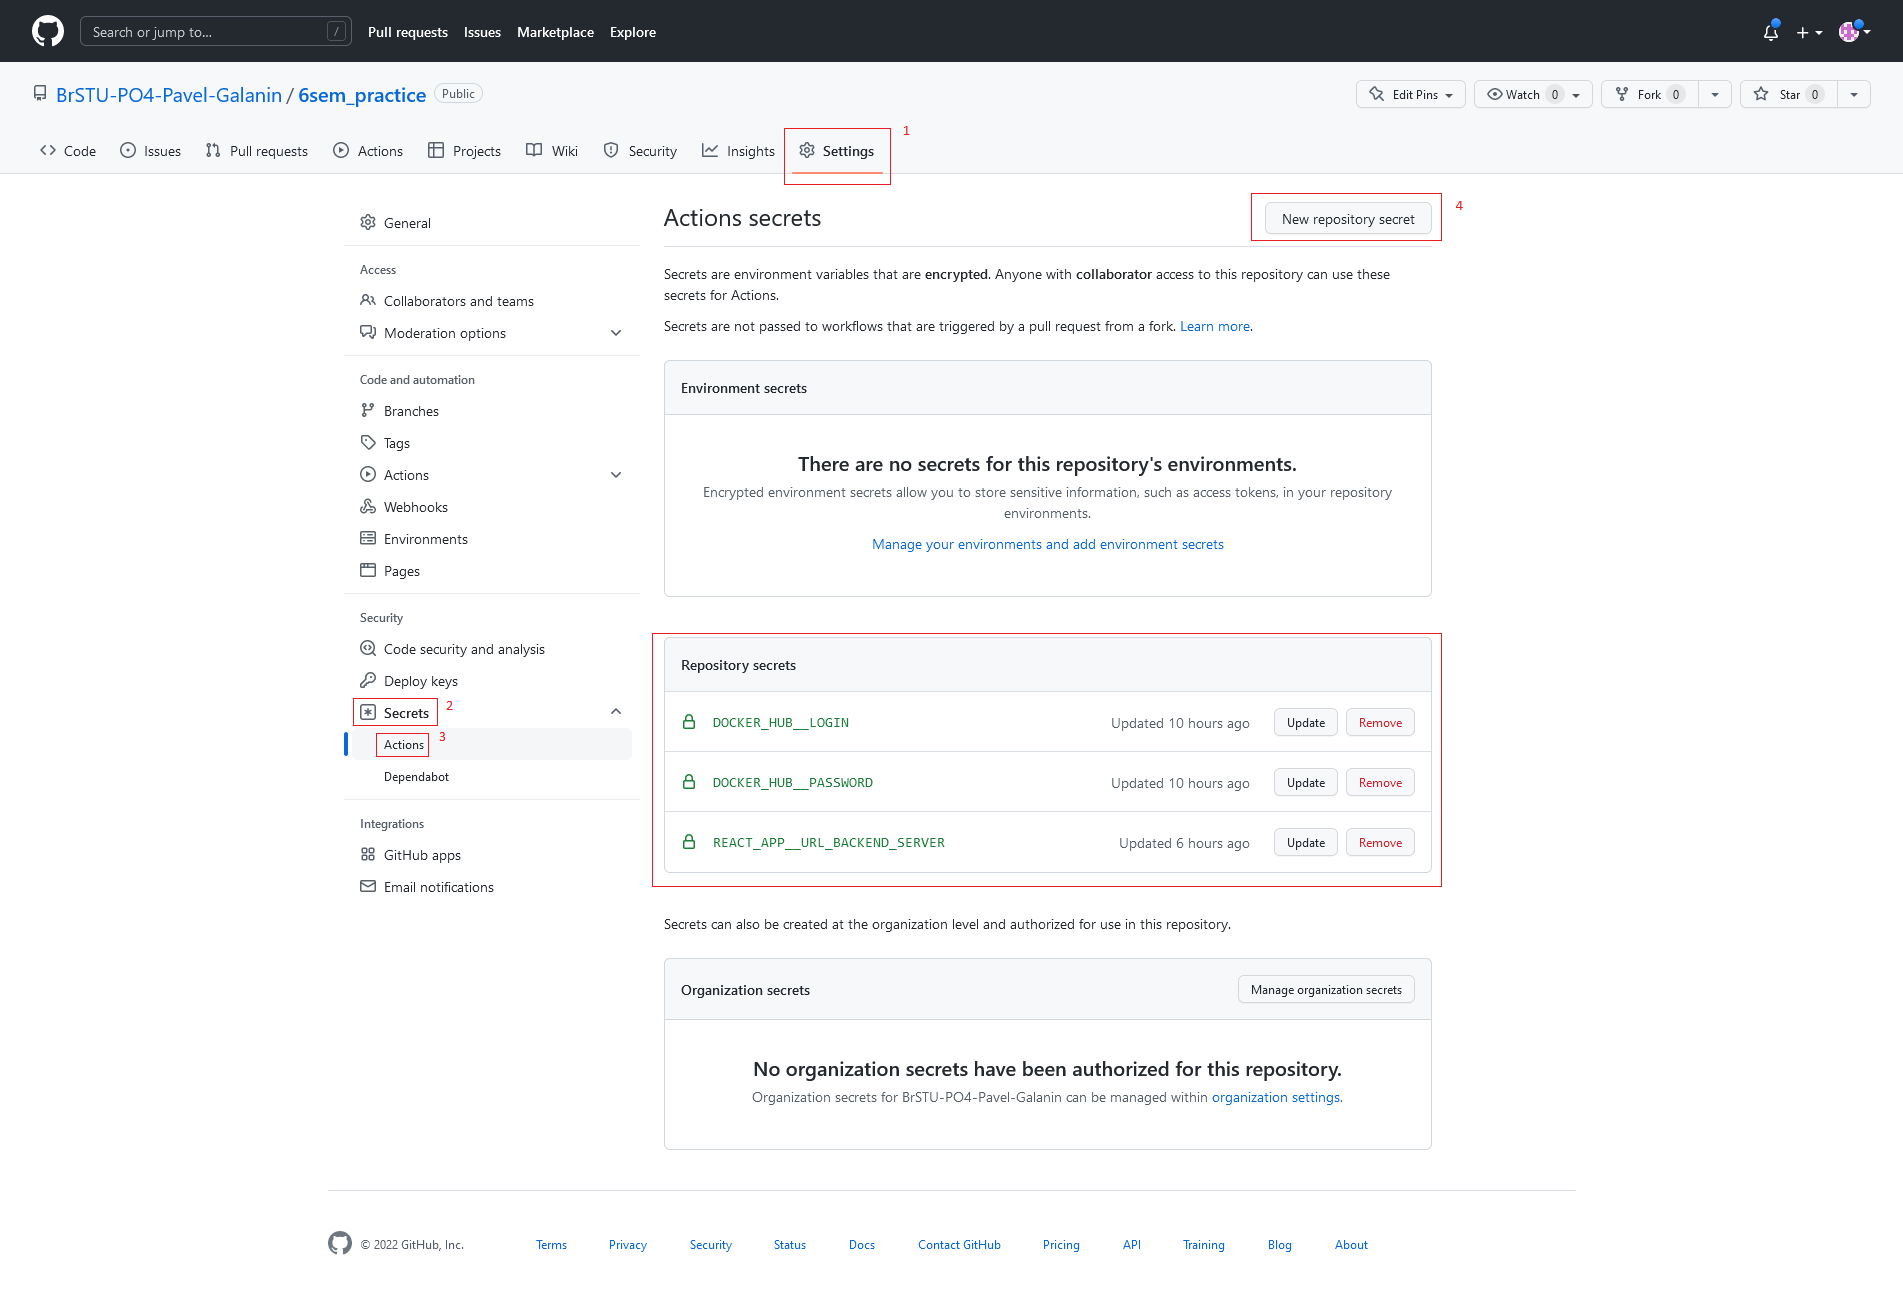
\includegraphics[width=18cm]
  {images/screenshots/GitHubSecrets.png}

  \caption{Добавление секретов (env в браузере)}
  \label{fig:GitHubSecrets}
\end{figure}

\begin{figure}[!h]
  \centering

  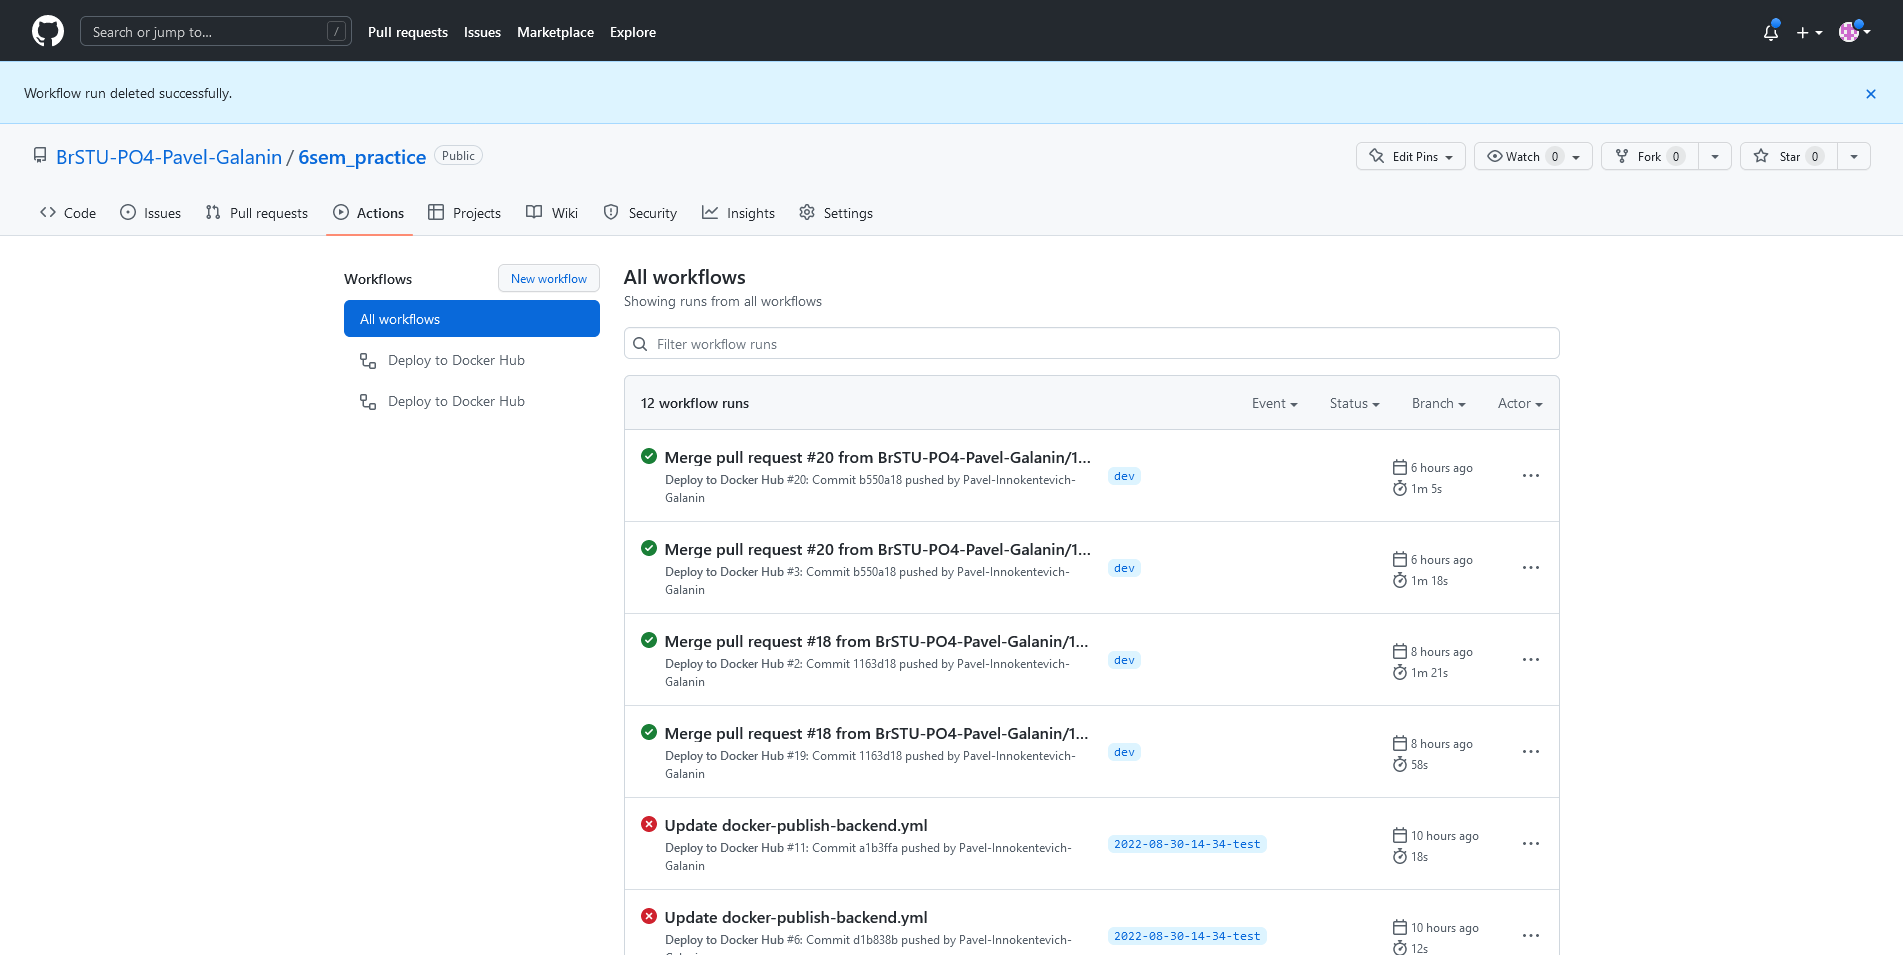
\includegraphics[width=18cm]
  {images/screenshots/GitHubActions.png}

  \caption{Остеживание сборки}
  \label{fig:GitHubActions}
\end{figure}

\newpage
\subsection{Запуск Docker образов на сервере Ubuntu}

Подключаемся к Ubuntu командой: ssh имя\_пользователя@ip\_адрес, вводим пароль,
затем пишем следующие команды:

\begin{itemize}
  \item sudo apt update
  \item sudo apt install git docker.io docker-compose -y
  \item git clone https://github.com/BrSTU-PO4-Pavel-Galanin/6sem\_practice
  \item cd 6sem\_practice/prod
  \item cp .env.example .env
  \item docker-compose up -f
  \item docker-compose ps
\end{itemize}

\lstinputlisting[]{../prod/.env.example}

\lstinputlisting[]{../prod/docker-compose.yml}

\lstinputlisting[]{../prod/docker.backend.run.sh}

\lstinputlisting[]{../prod/nginx.conf}
